\section{Residues}

\begin{definition}
    Let $f$ be an analytic functioin with Laurent series about the point $z=a$
    \begin{equation*}
        f(z)=\sum_{n=-\infty}^\infty{a_n(z-a)^n}
    \end{equation*}
    where the point $z=a$ is an isolated singularity. We define the
    \textbf{residue} of $f$ at  $a$ to be the term  $a_{-1}$, and write
    $\Res{(f,a)}$.
\end{definition}

\begin{theorem}[The Residue Theorem]\label{5.2.1}
    Let $f$ be a complex-valued function analytic on a region $U$, except at the
    isolated singularities  $a_1, \dots, a_m$. If $\y$ is a closed rectifiable
    nullhomologus path in  $U$, not passing through any of the $a_k$; that is
    $a_k \notin \{\y\}$ for all $1 \leq k \leq m$, then
    \begin{equation*}
        \frac{1}{2i\pi}\int_\y{f}=\sum_{k=1}^m{W(\y,a_k)\Res{(f,a_k)}}
    \end{equation*}
\end{theorem}
\begin{proof}
    Let $m_k=W(\y,a_k)$ for all $1 \leq k \leq m$, and choose  $r_1, \dots,
    r_m>0$ such that the collection of open ball $\{B(a_k,r_k)\}$ is pairwise
    disjoint from $\{\y\}$, and contained in $U$. Let
    $\y_k(y)=a_k+r_k\exp{(-2i\pi{m_kt})}$ on $0 \leq t \leq 2\pi$. Then for  $1
    \leq j \leq m$, we have
     \begin{equation*}
         W(\y,a)+\sum_{k=1}^m{W(\y_k,a_k)}=0 \text{ for all } a \notin
         \com{U}{\{a_1, \dots, a_m\}}
    \end{equation*}
    Now, since $f$ is analytic on  $\com{G}{\{a_1,\dots,a_m\}}$, by Cauchy's
    integral formula
    \begin{equation*}
        \int_\y{f}+\sum_{k=1}^m{\int_{\y_k}{f}}=0
    \end{equation*}
    Now, if $f(z)=\sum_{-\infty}^\infty{b_n(z-a_k)^n}$ is the Laurent series
    expansion of $f$ about the point  $z=a_k$, then the series converges
    uniformly on the boundry  $\partial{B(a_k,r_k)}$, so that
    \begin{equation*}
        \int_{\y_k}{f}=\sum_{-\infty}^\infty{b_n\int_{\y_k}{(z-a_k)^n \ dz}}
    \end{equation*}
    For $n \neq -1$, the integral  $\int_\y_k{(z-a_k)^n \ dz}=0$, and since
    $(z-a_k)^n$ has a primitive, we observe that
    \begin{equation*}
        b_{-1}\int_{\y_k}{(z-a_k)^{-1} \ dz}=2i\pi{W(\y,a_k)\Res{(f,a_k)}}
    \end{equation*}
    That is,
    \begin{equation*}
        \int_\y{f}-2i\pi\sum_{k=1}^m{W(\y_a_k)\Res{(f,a_k)}}=0
    \end{equation*}
\end{proof}

\begin{lemma}\label{5.2.2}
    Let $f$ be an analytic function with a pole of order $m$ at the point $z=a$,
    and let  $g(z)=(z-a)^mf(z)$. Then
    \begin{equation*}
        \Res{(f,a)}=\frac{g^{(m-1)}(a)}{(m+1)!}
    \end{equation*}
\end{lemma}
\begin{proof}
    If $f$ has a pole of order  $m$ at  $z=a$, then  $g$ has a removable
    singularity at  $z=a$, with  $g(a) \neq 0$. Let
    \begin{equation*}
        g(z)=b_0+b_1(z-a)+\dots
    \end{equation*}
    Then for any $z$ in an open ball about  $a$
    \begin{equation*}
        f(z)=\frac{b_0}{(z-a)^m}+\dots+\frac{b_{m-1}}{z-a}+
        \sum_{k=0}^\infty{b_{m+k}(z-a)^k}
    \end{equation*}
    gives us the Laurent series expansion of $f$ about $z=a$ in a punctured ball
    about $z=a$. Then by definition of the residue,  $\Res{(f,a)}=b_{m-1}$, but
    notice that
    \begin{equation*}
        b_{m-1}=\frac{g^{(m-1)}(a)}{(m+1)!}
    \end{equation*}
\end{proof}
\begin{corollary}
    If $f$ has a simple pole at  $z=a$, then
    \begin{equation*}
        \Res{(f,a)}=g(a)=\lim_{z \xrightarrow{} a}{(z-a)f(z)}
    \end{equation*}
\end{corollary}

We conclude this section with examples of finding integrals via the residue
theorem.

\begin{example}\label{example_5.2}
    \begin{enumerate}
    \item[(1)] To compute
        \begin{equation*}
            \int_{-\infty}^\infty{\frac{x^2}{1+x^4} \ dx}
        \end{equation*}

        Let $f(z)=\frac{z^2}{1+z^4}$. Then $f$ has as its poles the $4$-th roots
        of  $-1$; i.e. all $\xi$ for which $\xi^4=-1$. That is,  $f$ has as its
        poles the roots  $\xi=\exp{it}$ where
        \begin{equation*}
            t=\frac{\pi}{4}, \frac{3\pi}{4}, \frac{5\pi}{4}, \text{ and } \frac{7\pi}{4}
        \end{equation*}
        Now, take
        \begin{equation*}
            \xi_n=\exp{i(\frac{\pi}{4}+(n-1)\frac{\pi}{2})} \text{ for } 1 \leq
            n \leq 4
        \end{equation*}
        Then each $\xi_n$ is a simple pole of  $f$, so choosing $\xi_1$ and
        $\xi_2$, we get the following residues
        \begin{equation*}
            \Res{(f,\xi_1)}=\frac{1-i}{4\sqrt{2}}=\frac{1}{4}\exp{(-\frac{i\pi}{4})}
            \text{ and }
            \Res{(f,\xi_2)}=\frac{-1-i}{4\sqrt{2}}=\frac{1}{4}\exp{(-\frac{3i\pi}{4})}
        \end{equation*}
        Let $R>1$, and choose  $\y=\y_1 \cup \y_2$ where
        \begin{align*}
            \y_1(t) &=  Re^{it} \text{ on } 0 \leq t \leq \pi  \\
            \y_2(t) &=  t   \text{ on } -R \leq t \leq R    \\
        \end{align*}

        \begin{figure}[h]
            \centering
            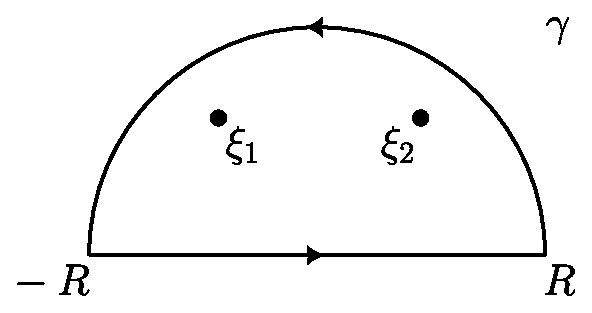
\includegraphics[scale=0.5]{Figures/Chapter5/contour_1.eps}
            \caption{}
            \label{figure_5.3}
        \end{figure}
        That is, $\y$ is the upper half ball of radius $R$. By the Residue
        theorem, we have
        \begin{equation*}
            \int_\y{f}=\Res{(f,\xi_1)}+\Res{(f,\xi_2)}= \frac{\pi}{\sqrt{2}}
        \end{equation*}
        observe also that
        \begin{equation*}
            \int_\y{f}=\int_{-R}^R{\frac{x^2}{1+x^4} \ dx}+
            i\int_0^\pi{\frac{R^3e^{3it}}{1+R^4e^{4it}} \ dt}
       \end{equation*}
       That is
        \begin{equation*}
            \int_{-R}^R{\frac{x^2}{1+x^4} \ dx}=\frac{\pi}{\sqrt{2}}-
            iR^3\int_0^\pi{\frac{e^{3it}}{1+R^4e^{4it}} \ dt}
       \end{equation*}
       Now, on $0 \leq t \leq \pi$, $1+R^4e^{4it}$ lies on the boundry
       $\partial{B(1,R^4)}$, hence
       \begin{equation*}
           |1+R^4e^{4it}| \geq R^4 \text{ and }
           \Big{|} iR^3\int_0^\pi{\frac{e^{3it}}{1+R^4e^{4it}} \ dt} \Big{|}
           \leq \frac{\pi{R^3}}{R^4-1}
       \end{equation*}
       Moreover, $\frac{x^2}{1+x^4} \geq 0$, for all $x \in \R$, so that
       \begin{equation*}
           \int_{-\infty}^\infty{\frac{x^2}{1+x^2} \ dx}=
           \lim_{R \xrightarrow{} \infty}{\int_{-R}^R{\frac{x^2}{1+x^4} \ dx}}=
           \frac{\pi}{\sqrt{2}}
       \end{equation*}

   \item[(2)] To compute
       \begin{equation*}
           \int_0^\infty{\frac{\sin{x}}{x} \ dx}
       \end{equation*}
       Notice that $f(z)=\frac{e^{iz}}{z}$ has a simple ple at $z=0$, so that
       $\Res{(f,0)}=1$. If $0<r<R$, let  $\y=\y_R \cup \l_1 \cup \y_r \cup \l_2$
       where
       \begin{align*}
           \y_R(t) &=   Re^{it} \text{ on } 0 \leq t \leq \pi   \\
           \l_1(t)  &=  t \text{ on } -R \leq t \leq -r \\
           \y_r(t)  &=  re^{-it} \text{ on } 0 \leq t \leq \pi  \\
           \l_2(t)  &=  t   \text{ on } r \leq t \leq R \\
       \end{align*}

       \begin{figure}[h]
           \centering
           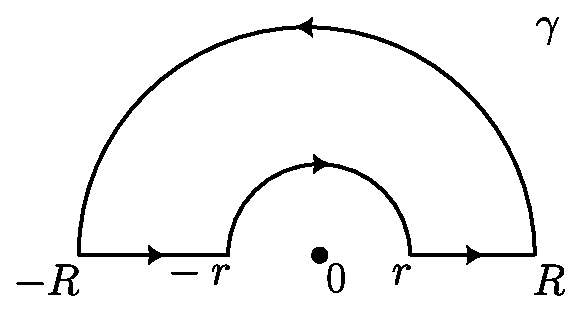
\includegraphics[scale=0.5]{Figures/Chapter5/contour_2.eps}
           \caption{}
           \label{figure_5.4}
       \end{figure}
       Now, notice that $0 \notin \Int{\y}$, so that $\y$ is nullhomotopic. By
       Cauchy's theorem, this give
       \begin{equation*}
           \int_\y{\frac{e^{iz}}{z} \ dz}=0
       \end{equation*}
       Now, we also have
       \begin{equation*}
           \int_\y{\frac{e^{iz}}{z} \ dz}=
           \int_r^R{\frac{e^{ix}}{x} \ dx}+
           \int_{\y_R}{\frac{e^{iz}}{z} \ dz}+
           \int_{-R}^{-r}{\frac{e^{ix}}{x} \ dx}+
           \int_{\y_r}{\frac{e^{iz}}{z} \ dz}
       \end{equation*}
       Now,
       \begin{equation*}
           \int_0^R{\frac{\sin{x}}{x} \
           dx}=\frac{1}{2i}\int_0^R{\frac{e^{ix}-e^{-ix}}{x} \ dx}
       \end{equation*}
       and
       \begin{equation*}
           \Big{|} \int_{\y_R}{\frac{e^{iz}}{z} \ dz} \Big{|} \leq
           \int_0^\pi{|\exp{(iRe{it})}| \ dt}=\int_0^\pi{\exp{(-R\sin{t})} \ dt}
       \end{equation*}
       For $\d>0$ small enough, whe have  $\exp{(-R\sin{t})} \leq
       \exp{(-R\sin{\d})}$, for any $\d<t<\pi-\d$. This gives that
       \begin{equation*}
           \Big{|} \int_{\y_R}{\frac{e^{iz}}{z} \ dz}
           \Big{|}<2\d+\pi\exp{(-R\sin{\d})}
       \end{equation*}
       Then for $\e>0$, choosing  $\d<\frac{\e}{3}$, there exists an $R_0$ such
       that $\exp{(-R\sin{\d})}<\frac{\e}{3\pi}$ for all $R>R_0$. This puts
       \begin{equation*}
       \lim_{R \xrightarrow{} \infty}{\int_{\y_R}{\frac{e^{iz}}{z} \ dz}}=0
       \end{equation*}
       Now, since $\frac{e^{iz}-1}{z}$ has a removable singularity at $z=0$, there
       exists an  $M>0$ such that  $|\frac{e^{iz}-1}{z}| \leq M$ for all
       $|z|<1$, hence
       \begin{equation*}
           \Big{|} \int_\y_r{\frac{e^{iz}-1}{z} \ dz} \Big{|} \leq \pi{rM}
       \end{equation*}
       so that
       \begin{equation*}
           \lim_{r \xrightarrow{} 0}{\int_\y_r{\frac{e^{iz}-1}{z} \ dz}}=0
       \end{equation*}
       now, notice also that $\int_{\y_r}{\frac{dz}{z}}=-i\pi$, so taht
       \begin{equation*}
           \lim_{r \xrightarrow{} 0}{\int_\y_r{\frac{e^{iz}}{z} \ dz}}=-i\pi
       \end{equation*}
       Then as $r \xrightarrow{} 0$, and $R \xrightarrow{} \infty$, we get
       \begin{equation*}
           \int_0^\infty{\frac{\sin{x}}{x} \ dx}=\frac{\pi}{2}
       \end{equation*}

   \item[(3)] To compute
       \begin{equation*}
           \int_0^\pi{\frac{dt}{a+\cos{t}}} \text{ for } a>1
       \end{equation*}

       Take $z=e^{it}$, then $\bar{z}=\frac{1}{z}$, and
       \begin{equation*}
           a+\cos{t}=a+\frac{1}{2}(z+\bar{z})=\frac{z^2+2az+1}{2z}
       \end{equation*}
       Thus
       \begin{equation*}
           \int_0^\pi{\frac{dt}{a+\cos{t}}}=\frac{1}{2}=
        \int_0^{2\pi}{\frac{dt}{a+\cos{t}}}=-i\int_\y{\frac{dz}{z^2+2az+1}}
       \end{equation*}
       where $\y$ is the unit circle. Now, $z^2+2az+1=(z-\a)(z-\b)$ where
       $\a=-a+\sqrt{a^2-1}$ and $\b=-a-\sqrt{a^2-1}$. Now, since  $a>0$,
       $|\a|<1$ and  $|\b|>1$ so only the simple pole $z=\a$ lies inside of
       $\y$. Then, by the residue theorem
       \begin{equation*}
           \int_\y{\frac{dz}{z^2+2az+1}}=\frac{i\pi}{\sqrt{a^2+1}}
       \end{equation*}
       so that
      \begin{equation*}
          \int_0^\pi{\frac{dt}{a+\cos{t}}}=\frac{\pi}{\sqrt{a^2+1}}
      \end{equation*}

      \item[(4)] To compute
          \begin{equation*}
              \int_0^\infty{\frac{\log{x}}{1+x^2} \ dx}
          \end{equation*}

          Consider the branch of the logarithm on the region
          \begin{equation*}
              U=\Big{\{} z \in \C : z \neq 0 \text{ and }
              -\frac{\pi}{2}<\arg{z}<\frac{3\pi}{2} \Big{\}}
          \end{equation*}
          now, if $z=|z|e^{it}$ with $-\frac{\pi}{2}<t<\frac{3\pi}{2}$, let
          \begin{equation*}
              L(z)=\log{|z|}+it
          \end{equation*}
          and let $\y$ be the path defined by figure \ref{figure_5.4}. Notice
          that
          \begin{equation*}
              L(z)=\begin{cases}
                        \log{x}, \text{ if } x>0    \\
                        \log{x}+i\pi, \text{ if } x<0
                  \end{cases}
          \end{equation*}
          hence we have
          \begin{equation*}
              \int_\y{\frac{L(z)}{1+z^2} \ dz}=
              \int_r^R{\frac{\log{x}}{1+x^2} \ dx}+
              iR\int_0^\pi{\frac{\log{R}+it}{1+R^2e^{2it}}e^{it} \dt}+
              \int_{-R}^{-r}{\frac{\log{|x|+i\pi}}{1+x^2} \ dx}+
              ir\int_0^\pi{\frac{\log{r}+it}{1+r^2e^{2it}}e^{it} \ dt}
          \end{equation*}
          Now, $\frac{L(z)}{1+z^2}$ has $z=i$ as its only simple pole inside of
           $\y$. Thus
           \begin{equation*}
               \Res{\frac{L(z)}{1+z^2},i}=\frac{1}{2i}(\log{|i|+\frac{i\pi}{2}})
           \end{equation*}
           so
           \begin{equation*}
               \int_\y{\frac{L(z)}{1+z^2} \ dz}=\frac{i\pi^2}{2}
           \end{equation*}
           Moreover,
           \begin{equation*}
               \int_r^R{\frac{\log{x}}{1+x^2} \ dx}+
               \int_{-R}^-r{\frac{\log{|x|+i\pi}}{1+x^2} \ dx}=
               2\int_r^R{\frac{\log{x}}{1+x^2} \
               dx}+i\pi\int_r^R{\frac{dx}{1+x^2}}
           \end{equation*}
           Letting $r \xrightarrow{} 0+$ and $R \xrightarrow{} \infty$, and
           noticing that
           \begin{equation*}
               \int_0^\infty{\frac{dx}{1+x^2}}=\frac{\pi}{2}
           \end{equation*}
           it follows that
           \begin{equation*}
               \int_0^\infty{\frac{\log{x}}{1+x^2} \ dx}=
               \frac{1}{2}\lim_{r \xrightarrow{} 0+}
                    {ir\int_0^\pi{\frac{\log{r}+it}{1+r^2e^{2it}}}e^{it} \ dt}-
                \frac{1}{2}\lim_{R \xrightarrow{} \infty}
                {iR\int_0^\pi{\frac{\log{R}+it}{1+R^2e^{2it}}}e^{it} \ dt}
           \end{equation*}
           Now, if $\p>0$, then
           \begin{equation*}
           \Big{|} \p\int_0^\pi{\frac{\log{\p}+it}{1+\p^2e^{2it}}e^{it} \ dt} \Big{|}
           \leq \frac{\p|\log{\p}|}{|1-\p^2|}\int_0^\pi{ \ dt}=
           \frac{\pi\p\log{\p}}{|1-\p^2|}+\frac{\pi^2\p}{2|1-\p^2|}
           \xrightarrow{} 0
           \end{equation*}
           as $\p \xrightarrow{} 0+$ or $\p \xrightarrow{} \infty$.

       \item[(5)] To compute
           \begin{equation*}
               \int_0^\infty{\frac{x^{-c}}{1+x} \ dx} \text{ for } 0<c<1
           \end{equation*}

           Consider the branch of $z^{-c}$ which has a branch point about $z=0$.

            \begin{figure}[h]
               \centering
               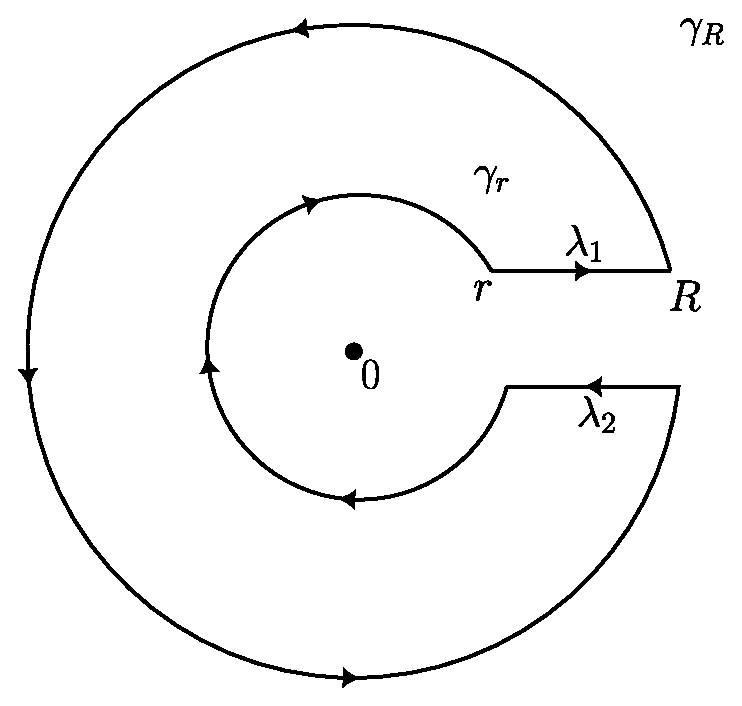
\includegraphics[scale=0.5]{Figures/Chapter5/contour_3.eps}
               \caption{}
               \label{figure_5.5}
           \end{figure}

           Let $U=\{z \in \C : z \neq 0 \text{ and } 0<\arg{z}<2\pi\}$ and
           define a branch of the logarithm on $U$ by
           \begin{equation*}
               L(re^{it})=\log{r}+it \text{ on } 0 \leq t \leq 2\pi
           \end{equation*}
           and for $z \in U$, put  $f(z)=\exp{-cL(z)}$. So $f$ is a branch of
           $z^{-c}$. Now, let $0<r<R$ and  $\d>0$, and consider the closed
           rectifiable path $\y=\y_R \cup \l_2 \cup \y_r \cup \l_1$ (see figure
           \ref{figure_5.5}) given by
           \begin{align*}
               \y_R  &:  |z|=R \text{ from } R+i\d \text{ to } R-i\d \\
               \l_2 &:  [R-i\d,r-i\d]   \\
               \y_r &:  |z|=r \text{ from } r-i\d \text{ to } r+i\d \\
               \l_1 &:  [r+i\d,R+i\d]
           \end{align*}
           notice then that $z=0$ does not lie inside of $\y$, so that  $\y$ is
           nullhomotopic. Moreover,  $-1$ is a pole ofr  $\frac{f(z)}{1+z}$, so
           that
           \begin{equation*}
               \Res{(\frac{f(z)}{1+z}),-1}=f(-1)=\exp{-i\pi{c}}
           \end{equation*}
           Now, we also have
           \begin{equation*}
               \inr_{\l_1}{\frac{f(z)}{1+z} \ dz}=
               \int_r^R{\frac{f(t+i\d)}{1+t+i\d} \ dt}
           \end{equation*}
           define $g(t,\d)$ on $[r,R] \times [0,\frac{\pi}{2}]$ by
           \begin{equation*}
               g(t,\d)=\Big{|} \frac{f(t+i\d)}{1+t+i\d}-\frac{t^{-c}}{1+t} \Big{|}
           \end{equation*}
           when $\d>0$, and  $g(t,0)$ is identically $0$, $g$ is continuous, and
           hence it must be uniformly continuous. If  $\e>0$, then there is a
           $\d_0>0$ for which
           \begin{equation*}
               |g(t,\d)-g(t',\d')|<\frac{\e}{R} \text{ whenever }
               (t-t')^2+(\d-\d')^2<\d_0^2
           \end{equation*}
           IN particular, $g(t,\d)<\frac{\e}{R}$ on $r \leq t \leq R$ and
           $\d<\d_0$. Thus
           \begin{equation*}
               \int_r^R{g(t,\d) \ dt}<\e \text{ for all } \d<\d_0
           \end{equation*}
           implying that
           \begin{equation*}
               \int_r^R{\frac{t^{-c}}{1+t} \ dt}=
               \lim_{\d \xrightarrow{} 0+}\int_{\l_1}{\frac{f(z)}{1+z} \ dz}
           \end{equation*}
           Similarly, since $L(\bar{z})=\bar{L(z)}$ we get
           \begin{equation*}
               -\exp{(2\pi{c})}\int_r^R{\frac{t^{-c}}{1+t} \ dt}=
               \lim_{\d \xrightarrow{} 0+}\int_{\l_1}{\frac{f(z)}{1+z} \ dz}
           \end{equation*}
           Letting $\d \xrightarrow{} 0+$, we get
           \begin{equation*}
           \begin{equation*}
               -2i\exp{(2\pi{c})}\int_r^R{\frac{t^{-c}}{1+t} \ dt}=
               \lim{\Big{(} \int_{\y_r}{\frac{f(z)}{1+z} \ dz}+
               \int_{\y_R}{\frac{f(z)}{1+z} \ dz} \Big{)}}
           \end{equation*}
           Now, let $\p>0$ and $\p \neq 1$. If $\y_\p:|z|=\p$ is the circle from
           $\sqrt{\p^2-\d^2}-i\d$ to $\sqrt{\p^2-\d^2}+i\d$, then
           \begin{equation*}
               \Big{|} \int_{\y_\p}{\frac{f(z)}{1+z} \dz} \Big{|} \leq
               \frac{\p^{-c}}{|1+\p|}2\pi\p
           \end{equation*}
           which implies that
           \begin{equation*}
               \Big{|} (2i\pi\exp{-i\pi{c}}-
               (1-\exp{-2i\pi{c}})\)\int_r^R{\frac{t^{-c}}{1+t} \ dt} \Big{|}
               \leq \frac{r^{-c}}{|1+r|}2\pi{r}+\frac{R^{-c}}{|1+R|}2\pi{R}
               \xrightarrow{} 0
           \end{equation*}
           as $r \xrightarrow{} 0+$ and $R \xrightarrow{} \infty$. THus we get
           \begin{equation*}
               2i\pi\exp{i\pi{c}}=
               (1-\exp{2i\pi{c}})\int_0^\infty{\frac{t^{-c}}{1+t}\ dt}
           \end{equation*}
           That is
           \begin{equation*}
            \int_0^\infty{\frac{t^{-c}}{1+t}\ dt}=\frac{\pi}{\sin{\pi{c}}}
           \end{equation*}
    \end{enumerate}
\end{example}
